 % !TEX root = ../imprimante3d.tex

\section{Matériel}

Ce chapitre décrit les différentes parties de l'imprimante et leur utilité. Encore une fois les illustrations montrent une Ultimaker mais les autres imprimantes ne sont pas si différentes.

\subsection{Contrôleur}

Le contrôleur est l'interface de l'imprimante. S'il n'y en a pas, cela signifie que l'imprimante se pilote directement depuis l'ordinateur. Un contrôleur permet à l'imprimante d'être totalement autonome. On peut également la configurer avant et pendant une impression. Lors d'une impression ce contrôleur nous indique la température des différents éléments, l'état d'avancement de l'impression et le temps écoulé.

\begin{figure}[H]
	\centering
	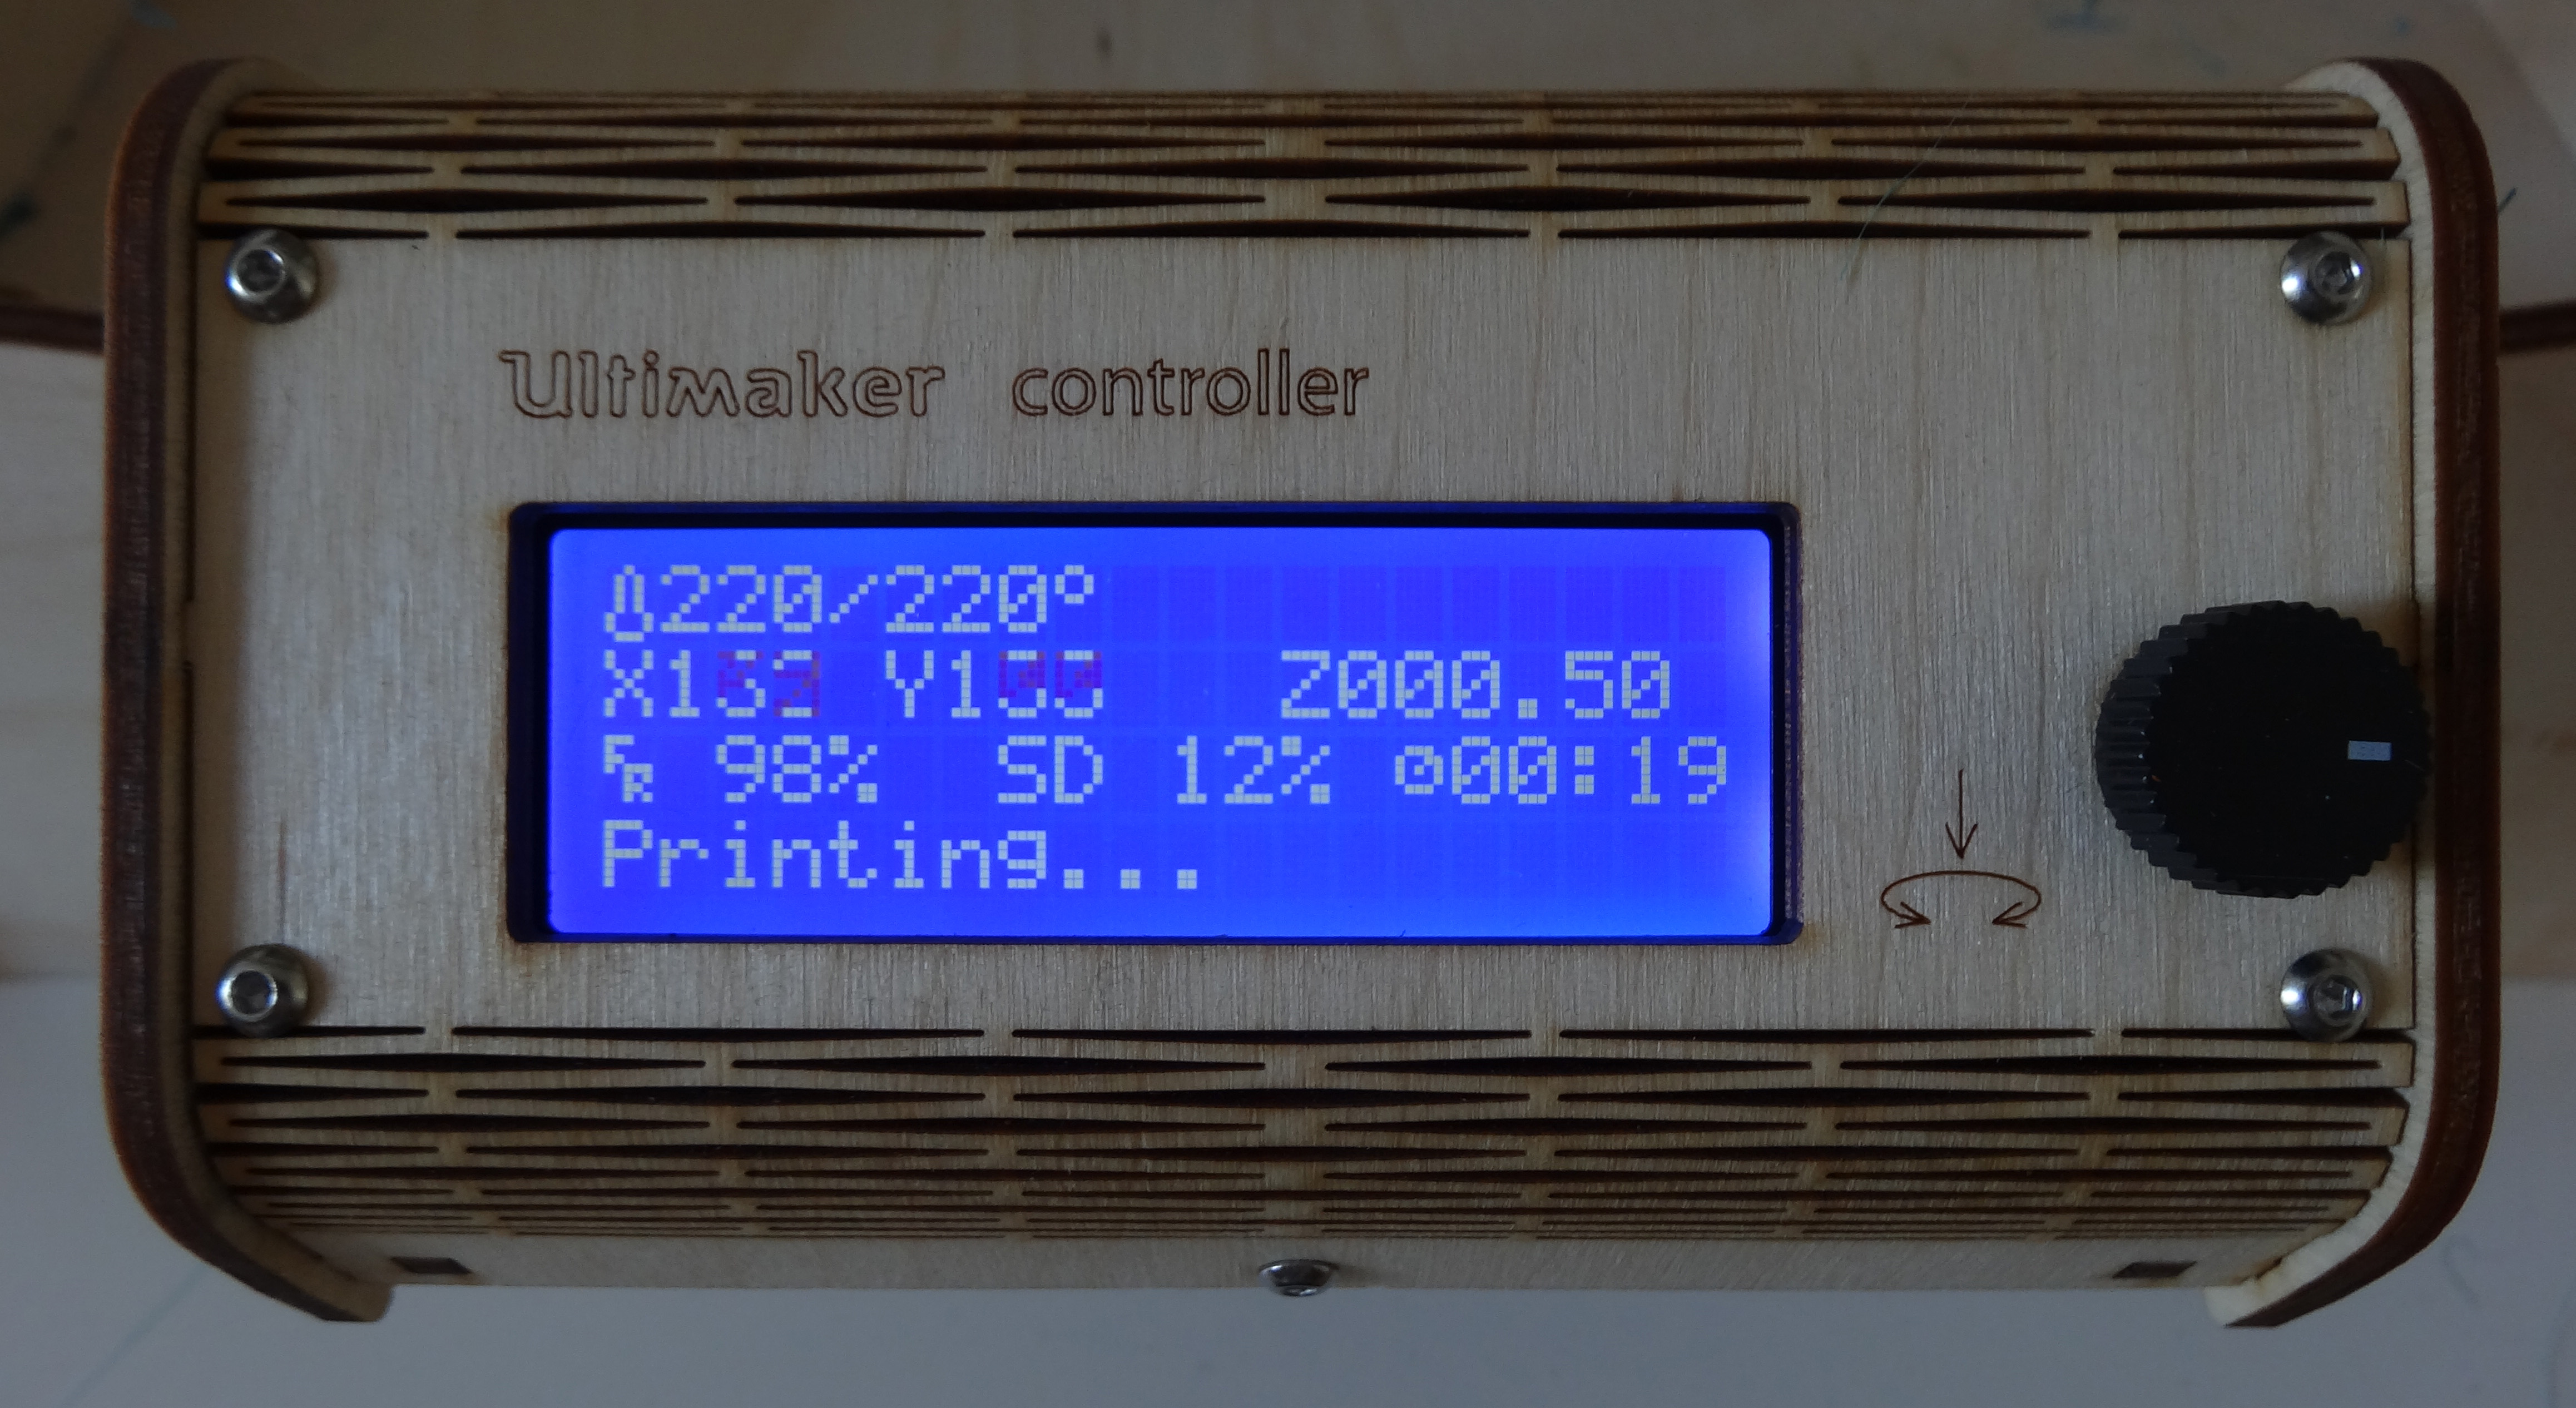
\includegraphics[width=50ex]{02_materiel/controller.jpg}  
	\caption{Contrôleur de l'Ultimaker V1}
	\label{fig:controller}
\end{figure}

\paragraph{} Concernant l'état d'avancement, il s'agit de l'avancement dans le fichier contenant le GCode (le code machine). Il ne faut pas prendre cette information trop sérieusement. Elle ne correspond pas au pourcentage de temps écoulé. C'est juste une indication. Pour connaitre ne approximation du temps d'impression, il faut regarder le temps indiqué dans les logiciels (même si celui-ci n'est pas forcément très précis).

\subsection{Tête d'impression}

La tête d'impression sert à faire fondre le filament et le déposer couche par couche. Elle fait usuellement $400\mu$ de diamètre. Le plateau doit être calibré de sorte à frôler la tête d'impression en tout points du plateau. Pour vérifier ceci, il suffit de faire un \emph{Auto Home} avec le contrôleur ou l'ordinateur de sorte à remettre l'imprimante à sa position de départ. Ensuite on déplace gentiment à la main la tête sur le plateau pour voir si le plateau est bien calibré. Si ce n'est pas le cas, il faut s'aider des vis dans les coins pour l'ajuster.

\begin{figure}[H]
	\centering
	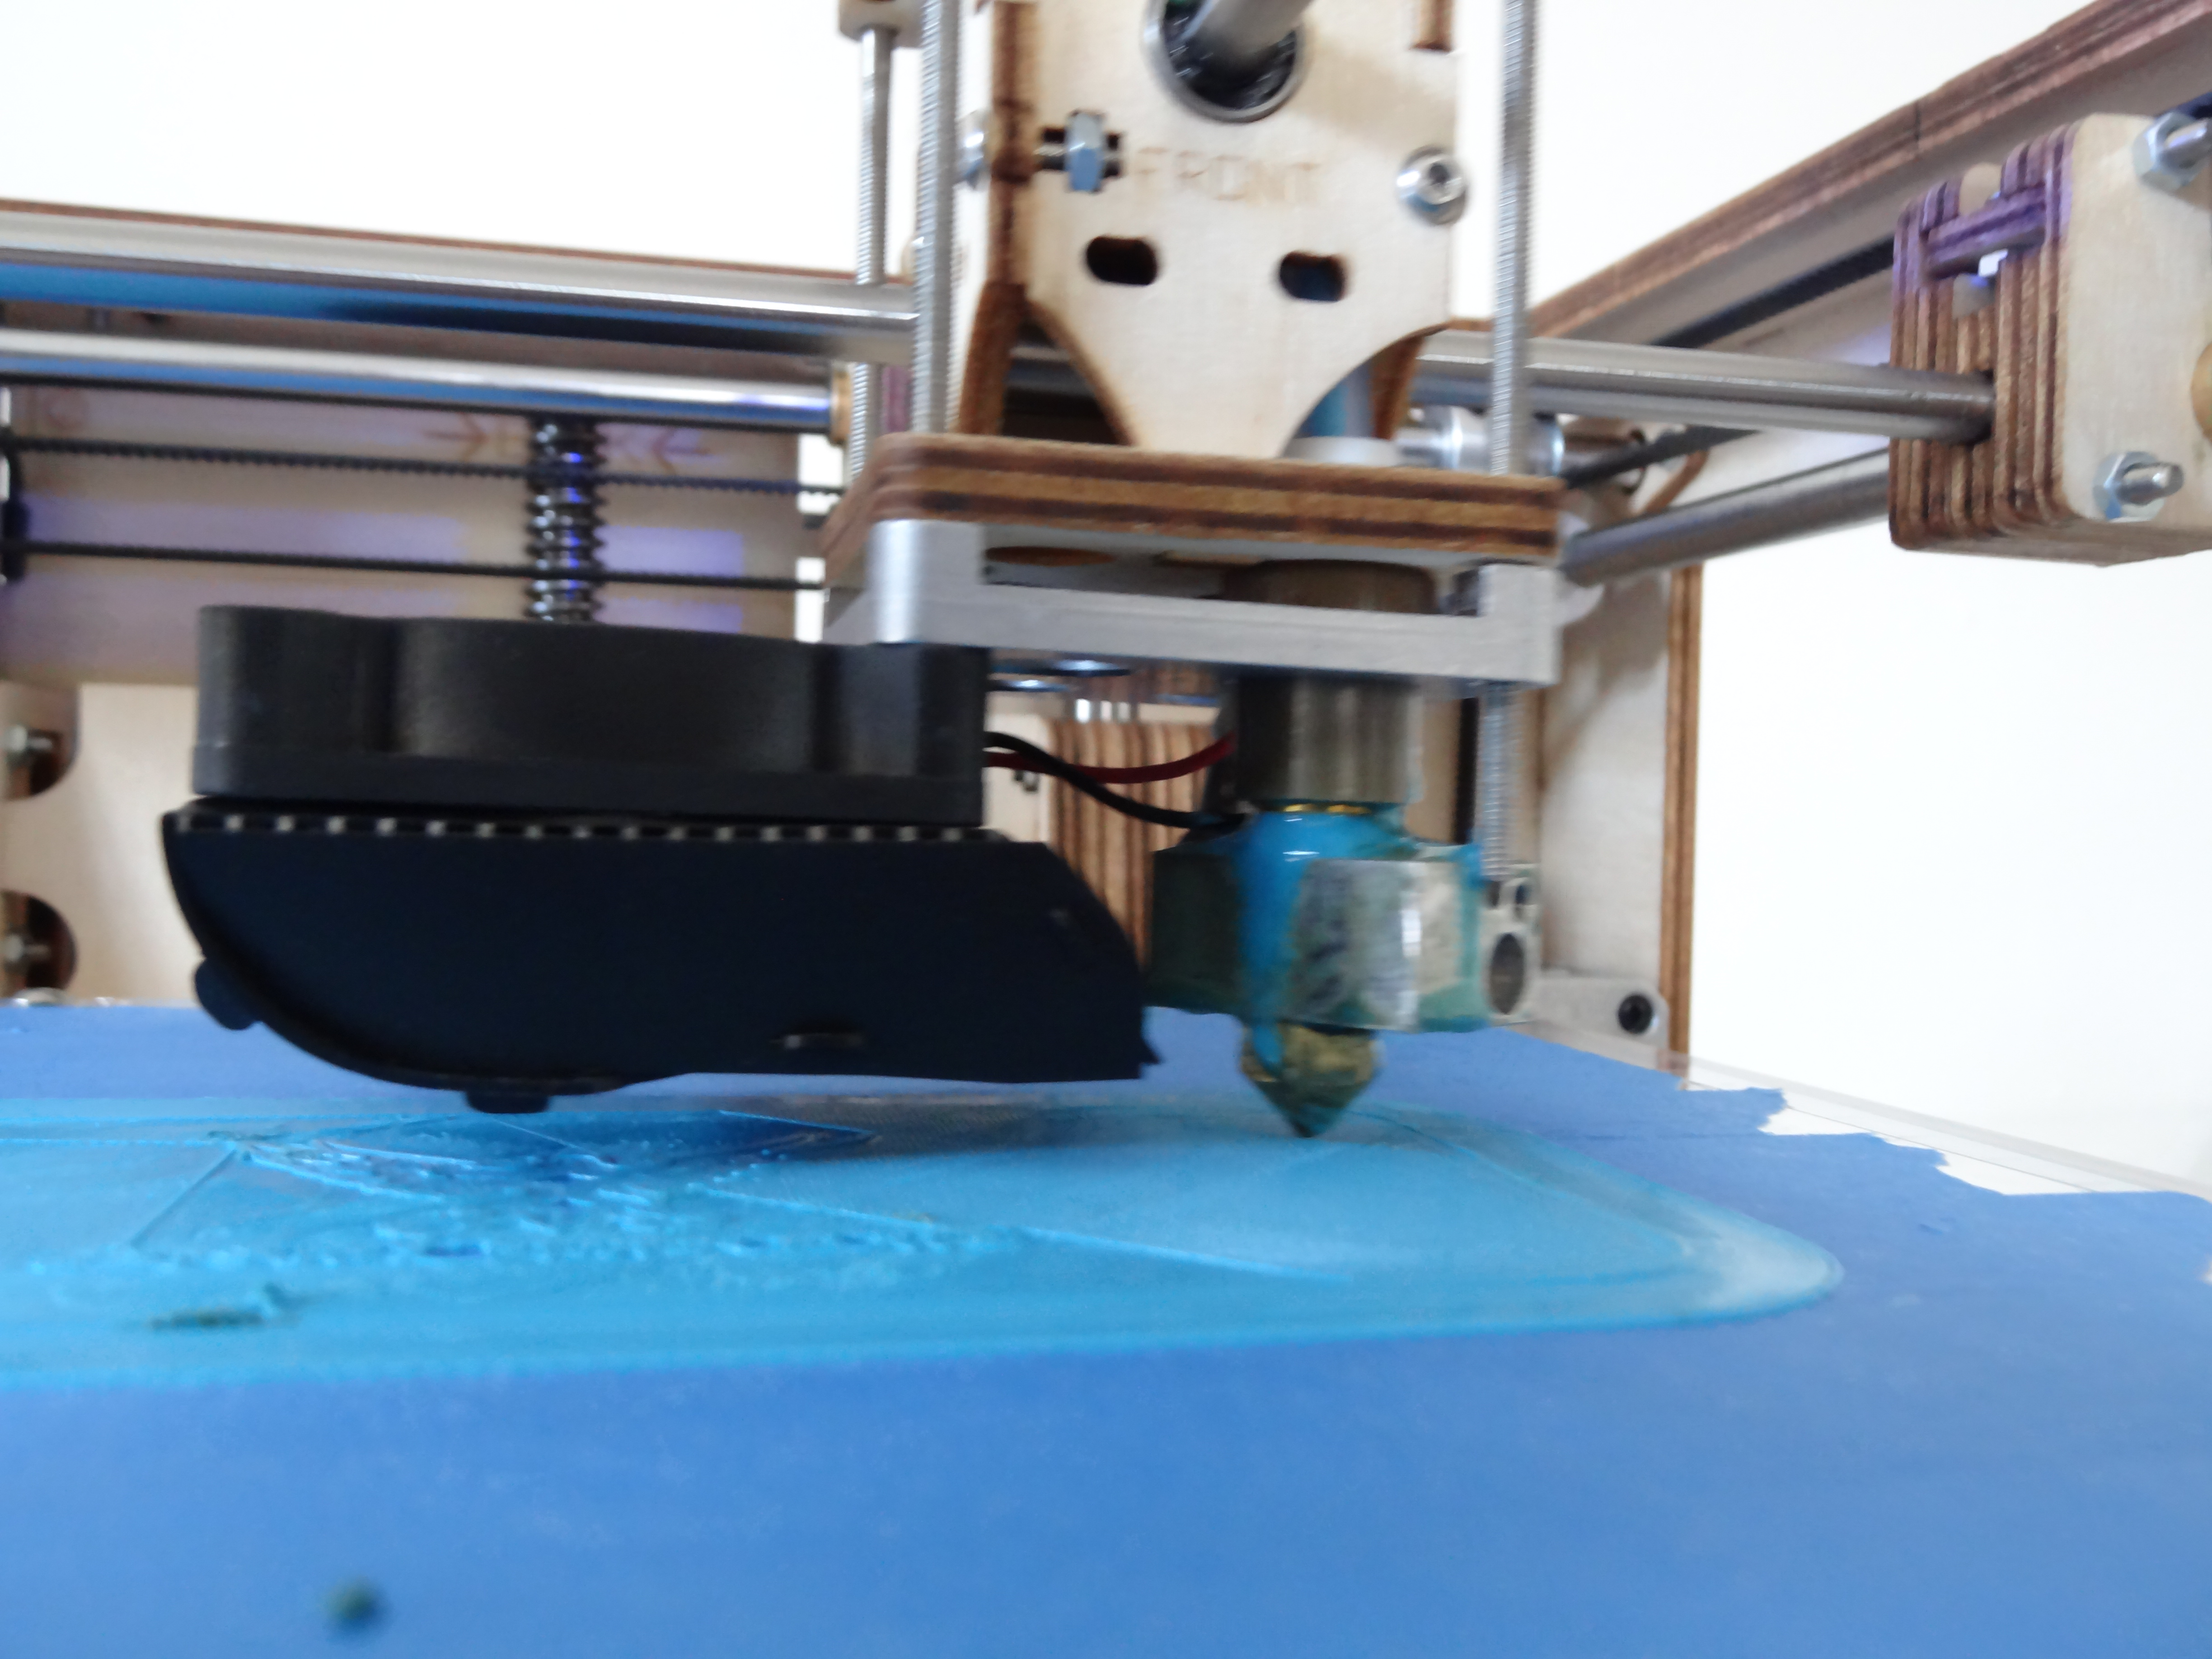
\includegraphics[width=50ex]{02_materiel/head1.jpg}  
	\caption{Tête d'impression de l'Ultimaker V1}
	\label{fig:head1}
\end{figure}

\subsection{Plateau}

\subsection{Scotch d'adhésion}

S'il n'y a pas de lit chauffant, le plateau est normalement recouvert d'un scotch aidant à l'adhésion de la pièce sur le plateau. Ce scotch se dégrade au fil du temps et doit être remplacé. Pour se faire, il suffit simplement d'enlever le plateau de l'imprimante et de remplacer le scotch à la main. Il y a des guides sur le plateau pour faciliter la découpe au cutter. Après cette opération, il ne faut pas oublier de recalibrer le plateau si cela s'avère nécessaire. A la fin d'une impression, la pièce peut être difficile à enlever. On peut s'aider d'un couteau pour faire décoller un coin de la pièce et le reste devrait venir assez facilement ensuite.

\subsection{Lit chauffant}

Le but du lit chauffant est de faire adhérer la matière au plateau tout au long de l'impression. Il ne faut surtout pas le désactiver en cours de route. La température du lit dépend de la matière que l'on imprime. Pour du PLA, il faut le mettre entre 60 et 70°C, mais pour de l'ABS, cela se situe plus autour des 100°C. A la fin de l'impression, il faut attendre que le lit refroidissent. Une fois que le lit est froid la pièce se décollera d'elle-même.

\subsection{Moteurs}

Les moteurs présents sur les imprimantes sont souvent des moteurs dits pas-à-pas. C'est-à-dire qu'ils ont des \emph{crans} tout les tant de degrés. Ils ont l'avantage d'être peu cher pour leur précision. 

 \paragraph{} Par contre il peut arriver qu'un moteur \emph{saute} ou loupe un ou plusieurs pas. Ceci est très mauvais, car l'imprimante ne saura pas qu'elle a glissé. L'imprimante envoie des commandes au moteur en lui disant le nombre de pas à avancer ou reculer. Si le moteur saute un pas, l'imprimante sera perdue et l'impression ne ressemblera à rien. On retrouve ce problème sur les CNC par exemple. Quand un moteur saute un pas, il faut un bruit spécial très distinct. Si cela arrive, il faut arrêter l'impression. Éventuellement graisser les axes et recommencer. L'environnement d'un Fablab est très poussiéreux, il peut donc arriver qu'un roulement devienne sale et qu'il faille le graisser (voir même le changer).

\subsubsection{Extrudeur}

Le moteur d'extrusion se trouve à l'arrière de l'Ultimaker. Pour les autres imprimantes, il se situe souvent sur la tête d'impression. Ce moteur pousse la matière dans la tête d'impression. Si le moteur n'est pas allumé, on peut sans autre tournée la rue pour pousser manuellement le filament. Comme on peut le voir sur la figure \ref{fig:extruder}, il y a une petite flèche pour indiquer le sens dans lequel tourner pour extraire de la matière.

\begin{figure}[H]
	\centering
	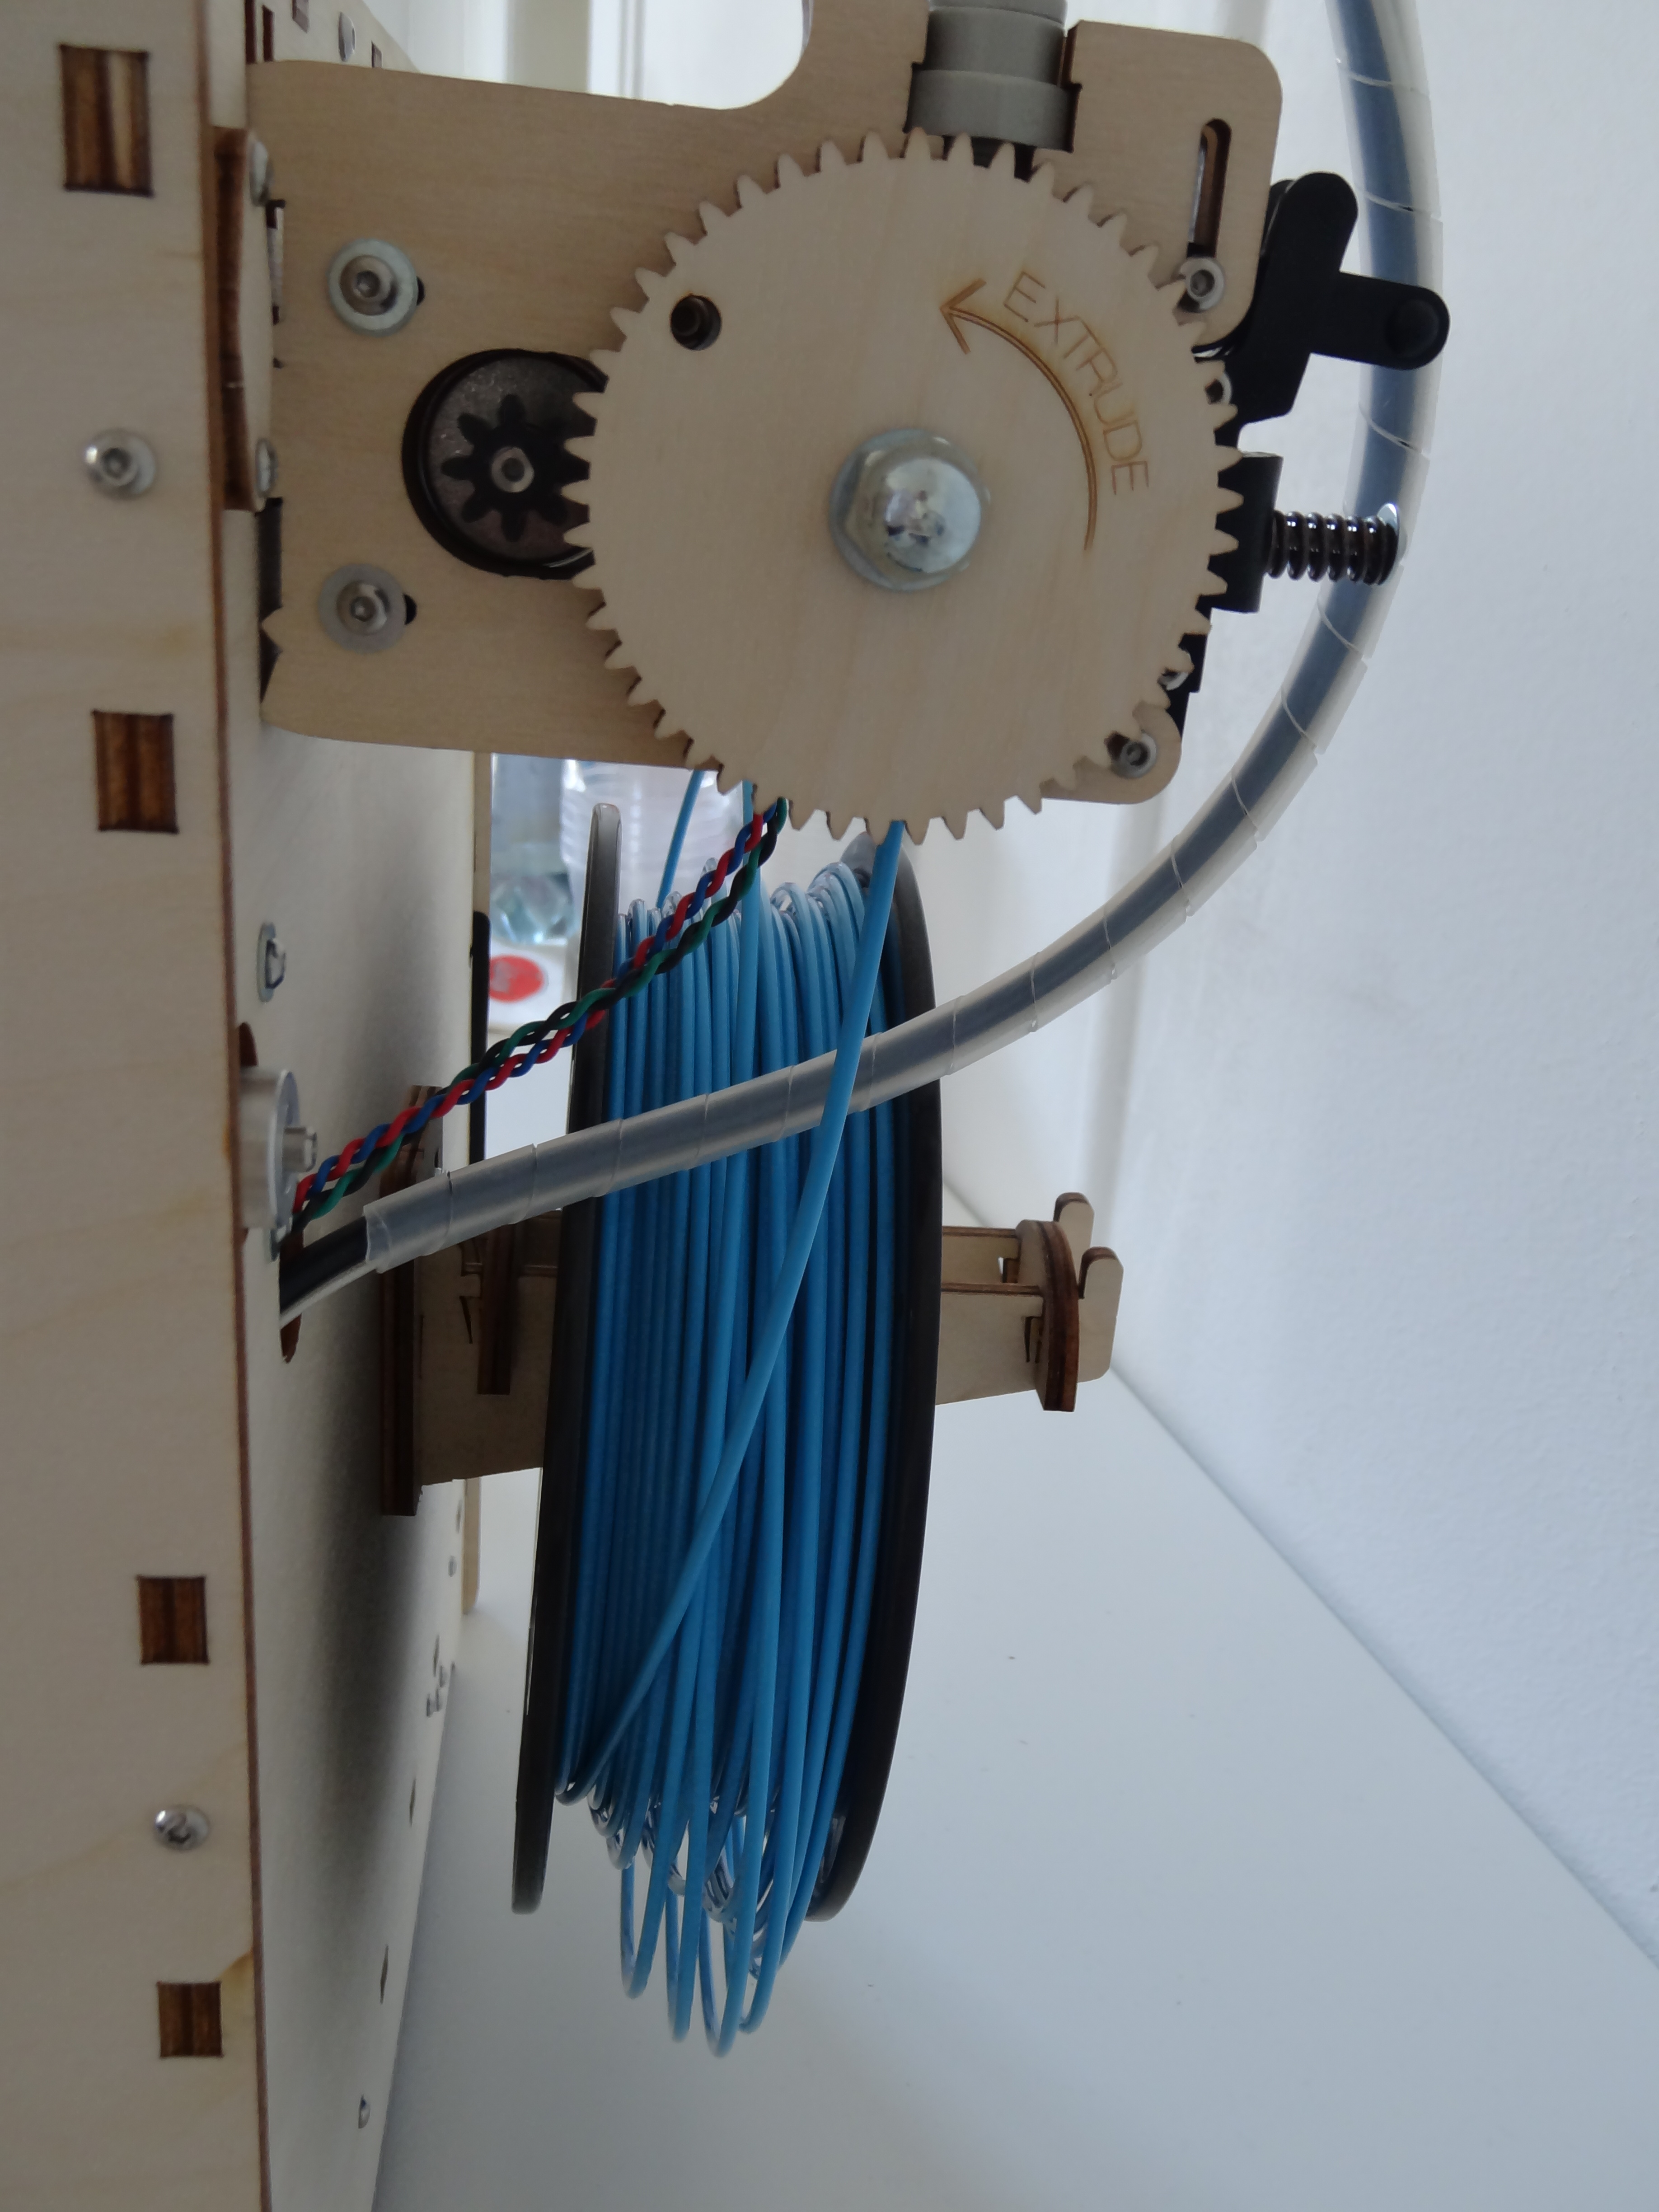
\includegraphics[width=50ex]{02_materiel/extruder.jpg}  
	\caption{Extrudeur et bobine sur l'Ultimaker V1}
	\label{fig:extruder}
\end{figure}

\subsubsection{Moteur x y z}

Ces moteurs servent à faire bouger la tête d'impression et le plateau. Sur l'Ultimaker, le plateau bouge en Z (en hauteur) et la tête en X (largeur) et Y (profondeur). Mais toutes les configurations sont possibles. Comme dit plus haut, il est possible que ces moteurs sautent des pas. Dans ce cas il faut graisser les roulements. Ne jamais graisser le moteur lui-même !

